\section{Meta Methods}
Meta Methods are using other methods to calculate their results, e\.g\. they can use pre generated heatmaps as an input.

\subsection{Network Dissection}
This method was introduced in 2017 by \fcite{Bau.2017} and is only applicable on convolutional networks. Their methods is divided into three steps: 
“
\begin{enumerate}
    \item  Identify a broad set of human-labeled visual concepts. 
    \item Gather hidden variables’ response to known concepts.
    \item Quantify alignment of hidden variable−concept pairs
\end{enumerate}
” \cite[2]{Bau.2017}
A human interpretable concept is often displayed by a combination of multiple variables and not only one. Nonetheless the paper measures the alignment between a single unit and a single interpretable concept. 
They did this, by finding pictures, that maximize the activation of a feature and then found the part of the picture, all of the pictures had in common (\cref{fig:NetworkDissection} figure 7).
\begin{figure*}[h]
    \center
    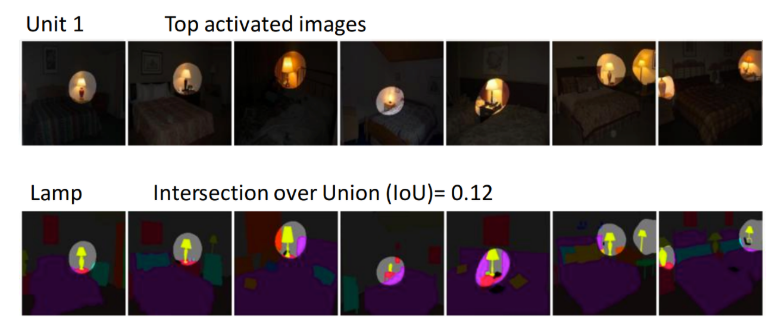
\includegraphics[width=\textwidth]{NetworkDissection}
    \caption{Network Dissection, \cite{Bau.2017}}
    \label{fig:NetworkDissection}
\end{figure*}

Interestingly they found, that lower layers of a CN interpret concepts like color or texture and higher layers more complex concepts like part or object, much like the human way of interpretation \cite{Bau.2017}.

\subsection{Concept Activation Vectors}
Concept Activation Vectors were published by \fcite{Kim.2018} in 2018. It aims to improve heatmaps in the point, that is it is only applicable to one picture at a time. The problem with that is, that even if a picture is of the same object, different parts of the object can be highlighted in the heatmap. This leads to confusion and mistrust.
\par
Their method measures the activation of a layer l produced of certain inputs. They then define a “concept activation vector” (or CAV) as the normal to a hyperplane separating examples without a concept and examples with a concept in the model’s activations” \cite[3]{Kim.2018}.
\par
A concept can be a special feature of a photo, e.g. a striped texture. So to compute such CAV, analysts needs a set of photos of striped objects and a set of random photos.
“Then, a binary linear classifier can be trained to distinguish between the layer activations of the two sets 
[...].
This classifier 
[...]
is a linear CAV for the concept” \cite[3]{Kim.2018}. Like this it can be found, which features exactly a NN learned.
In the paper they used a maximization technique in addition to sort the photos. Like this, the  underlying concept of a CAV can be visualized \cite{Kim.2018}.

\subsection{Spectral Relevance Analysis}
The \gls{spray} was first published in 2019 by \fcite{Lapuschkin.2019}. It aims to combine multiple explanations into one. It applies spectral clustering to pre generated heatmaps and identifies recurrent patterns. 
\par
“The identified features may be truly meaningful representatives of the object class of interest, or they may be co-occurring features learned by the model but not intended to be part of the class, and ultimately of the model’s decision process. Since SpRAy can be efficiently applied to a whole large-scale dataset, it helps to obtain a more complete picture of the classifier behavior and reveal unexpected or ‘Clever Hans’ type decision making” \cite[8]{Lapuschkin.2019}.
\par
\gls{spray} consists of four steps:
\begin{enumerate}
    \item The relevance maps for the dataset need to be calculated.
    \item Thereafter the relevance maps need to be resized to be in a uniform form.
    \item Spectral cluster analysis must be applied to the relevance maps. This groups classifier behaviors into clusters.
    \item Then interesting clusters can then be found via eigengap analysis.
\end{enumerate}
After that the results can be visualized \cite{Lapuschkin.2019}.
